\documentclass{article}
\usepackage{xcolor}
\newcommand{\red}{\color{red}}
\usepackage{tikz}
\usepackage[width=128mm]{geometry}
\pagestyle{empty}

\begin{document}

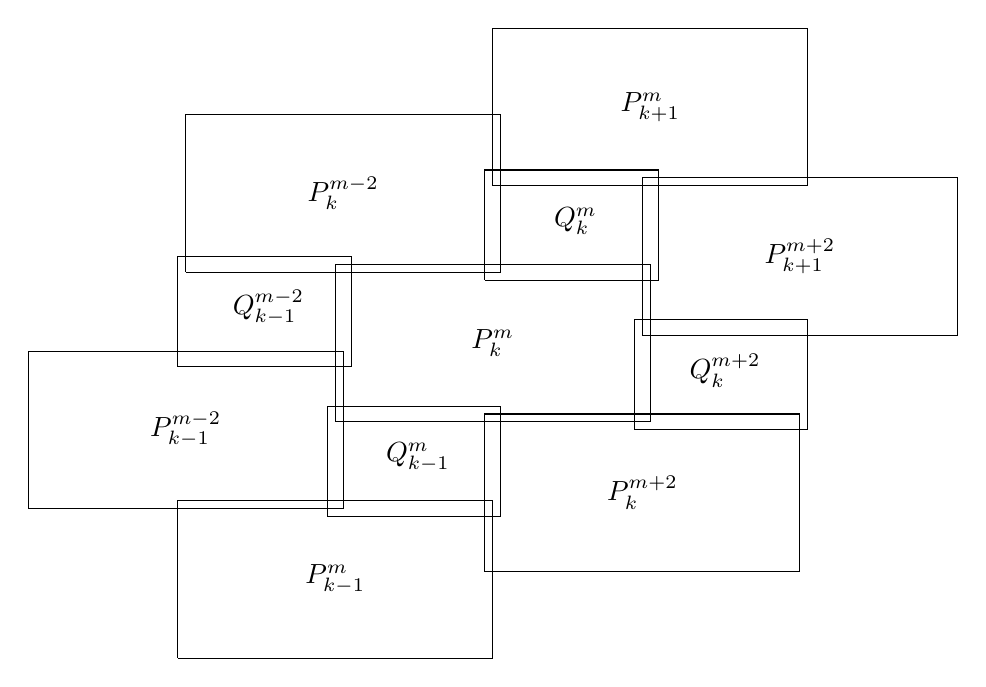
\begin{tikzpicture}
	\draw
	%% P column m-2
	(-1.9,1.9) -- +(4,0) -- +(4,2) -- +(0,2) -- +(0,0) +(2,1) node{$P_{k-1}^{m-2}$}
	(0.1,4.9) -- +(4,0) -- +(4,2) -- +(0,2) -- +(0,0) +(2,1) node{$P_{k}^{m-2}$}

	%% P column m
	(0,0) -- +(4,0) -- +(4,2) -- +(0,2) -- +(0,0) +(2,1) node{$P_{k-1}^{m}$}
	(2,3) -- +(4,0) -- +(4,2) -- +(0,2) -- +(0,0) +(2,1) node{$P_{k}^{m}$}
	(4,6) -- +(4,0) -- +(4,2) -- +(0,2) -- +(0,0) +(2,1) node{$P_{k+1}^{m}$}

	%% P column m+2
	(3.9,1.1) -- +(4,0) -- +(4,2) -- +(0,2) -- +(0,0) +(2,1) node{$P_{k}^{m+2}$}
	(5.9,4.1) -- +(4,0) -- +(4,2) -- +(0,2) -- +(0,0) +(2,1) node{$P_{k+1}^{m+2}$}

	%% Q column m-2
	(0,3.7) -- ++(0,1.4) -- ++(2.2,0) -- ++(0,-1.4) -- ++(-2.2,0) +(1.15,0.75) node{$Q_{k-1}^{m-2}$}

	%% Q column m
	(1.9,1.8) -- ++(0,1.4) -- ++(2.2,0) -- ++(0,-1.4) -- ++(-2.2,0) +(1.15,0.75) node{$Q_{k-1}^{m}$}
	(3.9,4.8) -- ++(0,1.4) -- ++(2.2,0) -- ++(0,-1.4) -- ++(-2.2,0) +(1.15,0.75) node{$Q_{k}^{m}$}

	%% Q column m+2
	(5.8,2.9) -- ++(0,1.4) -- ++(2.2,0) -- ++(0,-1.4) -- ++(-2.2,0) +(1.15,0.75) node{$Q_{k}^{m+2}$}

	;
\end{tikzpicture}

\end{document}
